% ****** Start of file apssamp.tex ******
%
%   This file is part of the APS files in the REVTeX 4.1 distribution.
%   Version 4.1r of REVTeX, August 2010
%
%   Copyright (c) 2009, 2010 The American Physical Society.
%
%   See the REVTeX 4 README file for restrictions and more information.
%
% TeX'ing this file requires that you have AMS-LaTeX 2.0 installed
% as well as the rest of the prerequisites for REVTeX 4.1
%
% See the REVTeX 4 README file
% It also requires running BibTeX. The commands are as follows:
%
%  1)  latex apssamp.tex
%  2)  bibtex apssamp
%  3)  latex apssamp.tex
%  4)  latex apssamp.tex
%
\documentclass[
reprint,
superscriptaddress,
%groupedaddress,
%unsortedaddress,
%runinaddress,
%frontmatterverbose, 
%preprint,
showpacs,
%preprintnumbers,
%nofootinbib,
%nobibnotes,
%bibnotes,
amsmath,
amssymb,
aps,
pra,
%prb,
%rmp,
%prstab,
%prstper,
%floatfix,
longbibliography
]{revtex4-1}

\usepackage{graphicx}% Include figure files
% \usepackage{dcolumn}% Align table columns on decimal point \SGc{We don't have any tables.}
% \usepackage{bm}% bold math \SGc{We don't seem to be using this.}
\usepackage{color}% Allows color text
\usepackage{hyperref}% add hypertext capabilities
%\usepackage[mathlines]{lineno}% Enable numbering of text and display math
%\linenumbers\relax % Commence numbering lines
\usepackage{ulem}% allows strike-out using sout
% \usepackage[caption=false]{subfig} \SGc{Don't have any subfigs.}

%\usepackage[showframe,%Uncomment any one of the following lines to test 
%%scale=0.7, marginratio={1:1, 2:3}, ignoreall,% default settings
%%text={7in,10in},centering,
%%margin=1.5in,
%%total={6.5in,8.75in}, top=1.2in, left=0.9in, includefoot,
%%height=10in,a5paper,hmargin={3cm,0.8in},
%]{geometry}


\newif\ifcmnt
%  Use \cmntfalse to not see comments when it is latex'ed
% \cmntfalse
%  Use \cmnttrue to see the comments
\cmnttrue 
\ifcmnt
    \providecommand{\aucmnt}[1]{#1}
    \providecommand{\editcolor}[2]{\textcolor{#1}{#2}}
\else
    \providecommand{\aucmnt}[1]{}
    \providecommand{\editcolor}[2]{#2}
\fi
\newcommand{\HV}[1]{\editcolor{blue}{#1}}
\newcommand{\HVc}[1]{\aucmnt{\editcolor{blue}{[HV: #1]}}}
\newcommand{\HVs}[1]{\aucmnt{\editcolor{blue}{\sout{#1}}}}
\newcommand{\SG}[1]{\editcolor{magenta}{#1}}
\newcommand{\SGs}[1]{\aucmnt{\editcolor{magenta}{\sout{#1}}}}
\newcommand{\SGc}[1]{\aucmnt{\editcolor{magenta}{[SG: #1]}}}
\newcommand{\LS}[1]{\editcolor{green}{#1}}
\newcommand{\LSs}[1]{\aucmnt{\editcolor{green}{\sout{#1}}}}
\newcommand{\LSc}[1]{\aucmnt{\editcolor{green}{[LS: #1]}}}
% find more colors at https://en.wikibooks.org/wiki/LaTeX/Colors#The_68_standard_colors_known_to_dvips


\newcommand{\rhotrue}{\rho_{\text{true}}}


\begin{document}

% \preprint{APS/123-QED}

\title{Quadrature Histograms in Maximum Likelihood Quantum State Tomography}% Force line breaks with \\
%\thanks{A footnote to the article title}%
\author{J. L. E. Silva}
\affiliation{Departamento de Engenharia de Teleinform\'atica, Universidade Federal do Cear\'a, Fortaleza, Cear\'a, 60440, Brazil}
\author{H. M. Vasconcelos}
\email{hilma@ufc.br}
\affiliation{Departamento de Engenharia de Teleinform\'atica, Universidade Federal do Cear\'a, Fortaleza, Cear\'a, 60440, Brazil}
\affiliation{Applied and Computational Mathematics Division, National Institute of Standards and Technology, Boulder, Colorado, 80305, USA}
\author{S. Glancy}
\affiliation{Applied and Computational Mathematics Division, National Institute of Standards and Technology, Boulder, Colorado, 80305, USA}

%\collaboration{MUSO Collaboration}%\noaffiliation

\date{\today}% It is always \today, today,
             %  but any date may be explicitly specified

\begin{abstract}
  Quantum state tomography aims to determine the quantum state of a
  system from measured data and is an essential tool for quantum
  information \SG{science}.  When dealing with continuous variable
  quantum states of light, QST is often done by measuring the field
  amplitudes at different optical phases using homodyne detection.
  The quadrature-phase homodyne measurement outputs a continuous
  variable, so to reduce the computational cost of tomography,
  researchers often discretize the measurements into histogram bin.
  We show that this can be done without significantly degrading the
  fidelity of the estimated state.  This paper tests different
  strategies for determining the histogram \SGs{bins}\SG{bin edges}.
  \SG{We show that computation time can be significantly reduced with
    little fidelity loss when the measurement operators corresponding
    to each histogram bin are integrated over the bin width.}
\end{abstract}

\pacs{
03.65.Wj, %State reconstruction, quantum tomography
03.67.-a, % Quantum information
42.50.Dv %Quantum state engineering and measurements in quantum optics
} % PACS, the Physics and Astronomy Classification Scheme.
%\keywords{Suggested keywords}%Use showkeys class option if keyword
                              %display desired
\maketitle

%\tableofcontents

\section{Introduction}
\label{intro}
Quantum information science and engineering \SGs{are at}\SG{have
  advanced to} the point where rudimentary quantum computers are
available in the laboratory and commercially~\cite{kandala2017,
  Linke2017, Monk2017, Denchev2016}.  However, further advancing
quantum technologies requires improvements in the fidelities of basic
operations.  Consequently, more precise and efficient reconstruction
and diagnostic tools used to estimate quantum states~\cite{Vogel1989,
  Smithey1993, Dunn1995, Banaszek1999, Banaszek2000, White2002,
  Ourjoumtsev2007, Neergaard2006}, processes~\cite{Chuang1997,
  Poyatos1997, Altepeter2003, Dariano1998, Nielsen1998, Mitchell2003,
  Obrien2004,Kupchak2015}, and measurements~\cite{Luis1999,
  Fiurasek2001, Dariano2004, Lundeen2009} are essential.  \SGc{joining
  paragraphs}Quantum \SGs{tomography}\SG{tomographic} techniques for
optical quantum states of light \SGs{has}\SG{have} become \SGs{a}
standard tool\SG{s} because quantum light sources are essential for
implementations of continuous-variable (CV) quantum computation
\SG{and communication}~\cite{Lloyd1999, Gottesman2001, Bartlett2002,
  Jeong2002, Ralph2003}.  These source are also extensively exploited
in quantum cryptography~\cite{Ralph1999, Hillery2000, Silberhorn2002,
  Pirandola2008, Luiz2017}, quantum metrology~\cite{Eberle2010,
  Demkowicz2013}, state teleportation~\cite{Vaidman1994,
  Braunstein1998, He2015}, dense coding~\cite{Braunstein2000, Lee2014}
and cloning~\cite{Cerf2000, Braunstein2001}.

In \SG{the} quantum state tomography \SG{studied here},
\SGs{we}\SG{one} performs a measurement on each member of a collection
of quantum systems, prepared in the same unknown state. \SG{Each
  system is measured in a basis chosen from a complete set of
  measurements.}  The goal is to estimate the unknown state from the
measurements results.  This estimation can be done by different
methods, but we study Maximum Likelihood Estimation (MLE), which finds
among all possible states, the one that maximizes the probability of
obtaining the observed data.

Quantum homodyne tomography is one of the most popular optical
tomography techniques available~\cite{Lvovsky2004}. It rapidly became
a versatile tool and has been applied in many different quantum optics
experimental settings since it was proposed by Vogel and Risken in
1989~\cite{Vogel1989} and first implemented by Smithey \textit{et al.}
in 1993~\cite{Smithey1993}. This technique permits one to characterize
an optical quantum state by analyzing multiple phase-sensitive
measurements of the field quadratures.

A homodyne measurement generates a continuous value.  \SG{It is a
  popular practice to discretize the measurement result, because this
  can considerably reduce the size of the data and expedite the
  reconstruction calculation.  However the discretization necessarily
  loses information contained in the original measurements.}
\SGs{Although discretization is not absolutely necessary, it is a
  popular practice, and we believe that the information lost by
  discretization may be insignificant. On the other hand,
  discretization of the data considerably reduces the size of the
  data, expediting the reconstruction algorithm.} How should we choose
a discretization strategy such that the bins are not too small nor too
large? Larger bins will reduce calculation time and memory, but
\SGs{the bins should not be too large in order to avoid a lack of
  resolution, making the histogram a poor representation of the
  underlying distribution}\SG{smaller bins will provide a better
  representation of the underlying distribution}.
 
In this paper, we use numerical experiments to simulate optical
homodyne tomography and perform maximum likelihood tomography on the
data with and without discretization. When choosing a quadrature bin
width, we use and compare two different strategies: Scott's
rule~\cite{Scott2010} and Leonhardt's formula~\cite{Leonhardt1996}.
The paper is divide as follow: we begin by reviewing maximum
likelihood in homodyne tomography in Section \ref{MLE}. Then, in
Section \ref{numerical-experiments}, we describe our numerical
experiments. Next, we discuss the estimation of the mean photon number
from the quadrature measurements in Section
\ref{sec-photon-estimation}. In Section \ref{results} we present our
results, and we make our concluding remarks in Section
\ref{conclusion}.

\section{Maximum likelihood in homodyne tomography}
\label{MLE}
Let us consider $N$ quantum systems, each prepared in an optical state
described by a density matrix $\rhotrue$. In each experimental trial
$i$, we measure the field quadrature of one of the systems at some
phase $\theta_i$ of a local oscillator, i.e.\ a reference system
prepared in a high amplitude coherent state.  Each measurement is
associated with an observable
$\hat{X}_{\theta_i} = \hat{X} \cos \theta_i + \hat{P} \sin \theta_i$,
where $\hat{X}$ and $\hat{P}$ are analogous to mechanical position and
momentum operators, respectively. For a given phase $\theta_i$, we
measure a quadrature value $x_i$, resulting in the data\SGs{ set}
$\{(\theta_i, x_i)| i = 1, \ldots, N\}$.

The outcome of the $i$-th measurement is associated with a
positive-operator-valued measure (POVM) element
$\Pi (x_i|\theta_i) = \Pi_i$. Given the data\SGs{ set}, the likelihood
of a candidate density matrix $\rho$ is
\begin{eqnarray}
  \mathcal{L} (\rho)= \prod_{i=1}^{N} \mathrm{Tr} (\Pi_i \rho),
  \label{eq-likelihood}
\end{eqnarray}
where $\mathrm{Tr}(\rho \Pi_i)$ is the probability, when measuring
with phase $\theta_i$, to obtain outcome $x_i$, according to the
candidate density matrix $\rho$.

MLE searches for the density matrix that maximizes the likelihood
in\SG{ Eq.}~(\ref{eq-likelihood}). \SGs{Equivalently, }It usually is
more convenient to maximize the logarithm of the likelihood (the
``log-likelihood''):
\begin{eqnarray}
  L (\rho) = \ln \mathcal{L} (\rho)= \sum_{i=1}^{N} \ln [\mathrm{Tr} (\Pi_i \rho)],
\end{eqnarray} 
which is maximized by the same density matrix as the likelihood. The
MLE is essentially a function optimization problem, and since the
log-likelihood function is concave, convergence to a unique solution
will be achieved by most iterative optimization methods.

In our numerical simulations, we use an algorithm for likelihood
maximization that begins with iterations of the $R\rho R$
algorithm~\cite{Rehacek2007} followed by iterations of a regularized
gradient ascent \SG{(RGA)} algorithm\SGs{ (RGA)}. \SGs{The main reason
  to}\SG{We } switch from one algorithm to another \SGs{is
  that}\SG{because} a slow-down is observed in the $R\rho R$ algorithm
after about $(t+1)^2/4$ iterations,\SG{where $t+1$ is the Hilbert
  space dimension}. In the RGA, $\rho^{(k+1)}$ is parametrized as
\begin{equation}
  \rho^{(k+1)}=\frac{\left(\sqrt{\rho^{(k)}}+A\right)\left(\sqrt{\rho^{(k)}}+A^{\dagger}\right)}{\mathrm{Tr}\left[\left(\sqrt{\rho^{(k)}}+A\right)\left(\sqrt{\rho^{(k)}}+A^{\dagger}\right)\right]},
  \label{eq-rho-k+1}
\end{equation}
where $\rho^{(k)}$ is the density matrix found by the previous
iteration, and $A$ may be any complex matrix of the same dimensions as
$\rho$. Eq.~(\ref{eq-rho-k+1}) ensures that $\rho^{(k+1)}$ is a
density matrix for any $A$. The matrix $A$ is chosen to maximize the
quadratic approximation of the log-likelihood subject to
$\text{Tr}(AA^{\dagger})\leq u$, where $u$ is a positive number
adjusted by the algorithm to guarantee that the log-likelihood
increases with each iteration. To halt the iterations, we use the
stopping criterion of \cite{Glancy2012},
$L(\rho_{\text{ML}})-L(\rho^{(k)})\leq 0.2$, where
$L(\rho_{\text{ML}})$ is the maximum of the log-likelihood.



\section{Numerical experiments}
\label{numerical-experiments}
\SGc{I don't love this section title, but I don't have a better idea
  right now.}  Our numerical experiments simulate single mode optical
homodyne measurements of two types of states: (1) superpositions of
coherent states of opposite phase $|-\alpha\rangle + |\alpha\rangle$
(called ``cat states'') and (2) squeezed vacuum states. \SGc{We might
  need to include Fock states here.} Each state is represented by a
density matrix $\rho_{\mathrm{true}}$ \SGs{truncated in a $n$ photon
  basis}\SG{represented in the photon number basis, truncated at $t$
  photons.}  \SG{To better simulate realistic experiments, these pure
  states are subject to some photon loss before measurement.} \SGc{Do
  we always use the same loss?  If so we can specify it here.  If not,
  we should specify in each case what loss is used.}

In order to calculate the probability to obtain homodyne measurement
outcome $x$, when measuring state $\rho_{\mathrm{true}}$ with phase
$\theta$, we need to represent $\Pi (x|\theta)$ in the \SGs{$n$}
photon number basis. If $|x\rangle$ is the photon number basis
representation of the x-quadrature eigenstate with eigenvalue $x$, and
$U(\theta)$ is the phase evolution unitary operator, then for an ideal
homodyne measurement, we have
$\Pi(x|\theta) = U(\theta)^{\dagger} |x\rangle \langle x|
U(\theta)$. To include photon \SGs{loss or}\SGc{Mathematically
  detector inefficiency is equal to loss, but we need to make a
  conceptual distinction between loss that is happening during the
  simulated state preparation and loss inside the homodyne detector.}
detector inefficiency, we replace the projector with
$\Pi(x|\theta) = \sum_{i=1}^{n} E_i(\eta)^{\dagger}
U(\theta)^{\dagger} |x\rangle \langle x| U(\theta) E_i(\eta)$, where
$\eta$ is the detection efficiency\SG{and $E_i(\eta)$ are the
  associated Kraus operators \cite{Lvovsky2004}}.  Typical
state-of-the-art homodyne detection systems have efficiency
$\eta \sim 0.9$, so we use this value in our simulations. Using this
strategy, we are able to correct for the \SGs{loss}\SG{detector
  inefficiency} as we estimate the state. We use rejection sampling
from the distribution given by $P(x|\theta)$ to guarantee random
samples of homodyne measurement results~\cite{Kennedy1980}.

To choose the phases at which the homodyne measurements are performed,
we divide the upper-half-circle evenly among $m$ phases between 0 and
$\pi$ and measure $N/m$ times at each phase, where $N$ is the total
number of measurements. In all simulations, we use $m=20$ and
$N = 20,000$. To secure a single maximum of the likelihood function,
we need an informationally complete set of measurement operators,
which can be obtained if we use $t+1$ different phases to reconstruct
a state that contains at most $t$ photons~\cite{Leonhardt1997}.

To quantify the similarity of the reconstructed state $\rho$ to the
true state $\rhotrue$ we use the fidelity
\begin{eqnarray}
  F = \mathrm{Tr} \sqrt{\rho^{1/2}\, \rhotrue \, \rho^{1/2}}.
\end{eqnarray}
\SGc{joining paragraphs} We report fidelities for four different
situations: (i) the state is reconstructed using the continuous values
of homodyne measurement results, that is without discretization; (ii)
the state is reconstructed with chosen bin widths (iii) the state is
reconstructed with bin widths given by Scott's rule~\cite{Scott2010};
and (iv) the state is reconstructed with bin widths suggested by
Leonhardt in~\cite{Leonhardt1997}. We only consider histograms with
contiguous bins of equal width\SGs{ for each phase}.

In 1979 Scott derived a formula recommending a bin width for
discretizing data sampled from a probability density function $f$ for
a single random variable $x$. The recommended bin width is
\begin{eqnarray}
  h^{\star} = \left[ \frac{6}{s \int_{-\infty}^{\infty} f'(x)^2 dx} \right]^{1/3},
  \label{eq-hstar}
\end{eqnarray}
where the first and second derivatives of $f$ must be continuous and
bounded and $s$ is the sample size. Because one does not know $f$ in
an experiment we assume a normal distribution. For a normal $f$ we
have
\begin{eqnarray}
  \int_{-\infty}^{\infty} f'(x)^2 dx = \frac{1}{4 \sqrt{\pi} \sigma ^3},
  \label{eq-intnormaldist}
\end{eqnarray}
where $\sigma$ is the distribution's standard deviation.  Combining
Eqs.~(\ref{eq-hstar}) and (\ref{eq-intnormaldist}), we obtain the
recommended bin width for a normal distribution:
\begin{eqnarray}
  h = 3.5 \, \sigma \, s^{-1/3}.
\end{eqnarray}
This formula is known as Scott's rule, and is optimal for \SG{for
  estimating $f$ (minimizing total mean-squared error) at} each phase
if the data is normally distributed. In our simulations we compute a
bin size separately for each phase's quadrature measurements, and we
use the \SGs{corrected}\SG{unbiased} sample standard deviation in
place of $\sigma$.

Although Scott's rule is optimal for each phase, it may not be optimal
for homodyne tomography because we are estimating the density matrix
rather than each phase's quadrature distribution individually.  Also
many interesting optical states do not have normal quadrature
distributions, for example our cat states.  In fact, one might expect
that the bin width should be related to the number of photons in a
quantum state because higher photon number states have more narrow
features in their quadrature distributions, which should not be
washed-out by the discretization.

Leonhardt states that if we desire to reconstruct a density matrix of
a state with $n$ photons, we need a bin width narrower than $q_n/2$,
where $q_n$ is given by
\begin{eqnarray}
  q_n = \frac{\pi}{\sqrt{2 n + 1}}.
  \label{eq-leonhardt}
\end{eqnarray}
This result was obtained \SGs{by using}\SG{from} a semiclassical
approximation for the amplitude pattern functions in quantum state
sampling~\cite{Leonhardt1996}. Leonhardt recommends using the maximum
photon number in Eq.~(\ref{eq-leonhardt}), however many states have no
maximum photon number, and whether a state has a \SGs{true }maximum
photon number is not possible to learn with certainty from tomography.
Instead, we have tested using the photon number \SG{$t$} at which the
reconstruction Hilbert space is truncated\SGs{ $M$} and an estimate of
the mean photon number $\overline{\langle \hat{n} \rangle}$ in
Eq.~(\ref{eq-leonhardt}).  The truncation $t$ must be chosen in
advance to be large enough that the probability that $\rhotrue$
contains more \SG{than $t$} photons \SGs{than the truncation limit} is
very small.  We estimate the mean photon number from the quadrature
measurements as described in the next section.



\section{Estimating mean photon number}
\label{sec-photon-estimation}
In order to use Leonhardt's advice for choosing the histogram bin
width, we need to estimate the mean number $\langle n \rangle$ of
photons in the measured state from the phase-quadrature data
set. \SG{We use the estimator given in
  Refs.~\cite{Hradil2,Munroe1996}}.  To \SGs{find an}\SG{to obtain
  this} estimator, we first compute the mean value of
$(\hat{X}_{\theta})^{2}$, averaged over $\theta$, treating $\theta$ as
if it is random and uniformly distributed between $0$ and $\pi$.
\begin{equation}
  \langle (\hat{X}_{\theta})^{2} \rangle = \langle \hat{X}^{2}\cos^{2}\theta + (\hat{X}\hat{P}+\hat{P}\hat{X})\cos\theta\sin\theta + \hat{P}^{2}\sin^{2}\theta \rangle
\end{equation}
The phase $\theta$ is independent of $\hat{X}$ and $\hat{P}$, so we
can compute the expectation over $\theta$ as
\begin{align}
  \langle (\hat{X}_{\theta})^{2} \rangle &= \Big\langle \int_{0}^{\pi} (\hat{X}^{2}\cos^{2}\theta + (\hat{X}\hat{P}+\hat{P}\hat{X})\cos\theta\sin\theta \nonumber \\
                                         & \qquad \qquad + \hat{P}^{2}\sin^{2}\theta) \mathrm{Prob}(\theta) \mathrm{d}\theta \Big\rangle \\
  \langle (\hat{X}_{\theta})^{2} \rangle &= \Big\langle \int_{0}^{\pi} (\hat{X}^{2}\cos^{2}\theta + (\hat{X}\hat{P}+\hat{P}\hat{X})\cos\theta\sin\theta \nonumber \\
                                         & \qquad \qquad + \hat{P}^{2}\sin^{2}\theta) \frac{1}{\pi} \mathrm{d}\theta \Big\rangle \\
                                         &= \frac{1}{2}\left\langle \hat{X}^{2} + \hat{P}^{2} \right\rangle.
\end{align}
Because the photon number operator is
\begin{equation}
  \hat{n} = \frac{1}{2}\left(\hat{X}^{2}+\hat{P}^{2}-1\right),
\end{equation}
we obtain
\begin{equation}
  \langle\hat{n}\rangle = \langle \hat{X}_{\theta}^{2}\rangle-\frac{1}{2}. 
\end{equation}
We estimate $\langle \hat{n} \rangle$ by computing the sample
mean of all quadrature measurements~\HV{\cite{Hradil2,Munroe1996}}:
\begin{equation}
  \overline{\langle \hat{n} \rangle} = \frac{1}{N} \sum_{i=1}^{N}x_{i}^{2} - \frac{1}{2}.
  \label{eq-photon-estimation}
\end{equation}
Note that when $\theta$ is uniformly distributed over $[0,\pi)$, the
\SG{individual} values of $\theta$ are not needed to compute
$\overline{\langle \hat{n} \rangle}$.



\section{Results}
\label{results}
\SG{To study the performance of various discretization strategies, we
  compute fidelities between the true state and the states estimated
  with the different strategies. Below $\rho_{\mathrm{ML2}}$
  represents the state estimated without discretization,
  $\rho_{\mathrm{Hist}}$ is estimated with histogram bins of specified
  width chosen arbitrarily, $\rho_{\mathrm{Scott}}$ is estimated with
  bin widths chosen according to Scott's rule, and
  $\rho_{\mathrm{Leonhardt}}$ is estimated with Leonhardt's bin
  widths.} \SGs{In our study, we compute the fidelities between the
  true state and (i) the density matrix reconstructed without
  discretization, $\rho_{\mathrm{ML2}}$; (ii) the density matrix
  reconstructed using histograms with chosen bin widths,
  $\rho_{\mathrm{Hist}}$; (iii) and the density matrix reconstructed
  using histograms with a bin width given by Scott's method,
  $\rho_{\mathrm{Scott}}$.}  \SGc{joining paragraphs}To make the
graphs below, for each choice of parameters, we simulate 100
tomography experiments, making 100 density matrix estimates.  The
graphs show the arithmetic mean of the 100 fidelities of the
reconstructed states. The error bars show the standard deviation of
the 100 fidelities.

%DISCUSSION OF FIGURE 1
Our first results are shown in
Fig.~\ref{fig-methods_fidelity_singledata}. The state considered is a
cat state with $\alpha = 1$, where $\alpha$ is the amplitude of the
coherent state in the superposition.  The state is reconstructed in a
Hilbert space truncated at $t=10$ photons. \SG{(The probability that
  the $\alpha=1$ state has more than 10 photons is ???.)} Scott's
method finds a different optimal bin width for each phase considered,
so we report the mean bin width averaged over the 20 phases in these
cases.  Here the mean bin width for Scott's method is $0.35$.  When
choosing a bin width, we go up to $0.34$, the value we obtain when we
use Eq.~(\ref{eq-leonhardt}) for $t=10$, the number of photons at
which we truncated the Hilbert space.  In all cases, each bin's
measurement operator represents the measurement as if it occurred at
the center of each bin. \SGc{joining paragraphs} In
Fig~\ref{fig-methods_fidelity_singledata}, each set of points
corresponds to a different data set. Our goal was to check that
different data sets would have similar behavior as we change the bin
size. As we can see in this figure, the highest \SGs{values of
  fidelity correspond to the case where}\SG{fidelities occur when} we
do not use discretization, as expected.  We also see that smaller bin
widths result in \SGs{the highest}\SG{higher} fidelities.  However,
even the largest bin widths tested result in a fidelity loss of only
0.005 compared to the raw data.

%FIGURE 1
\begin{figure}
  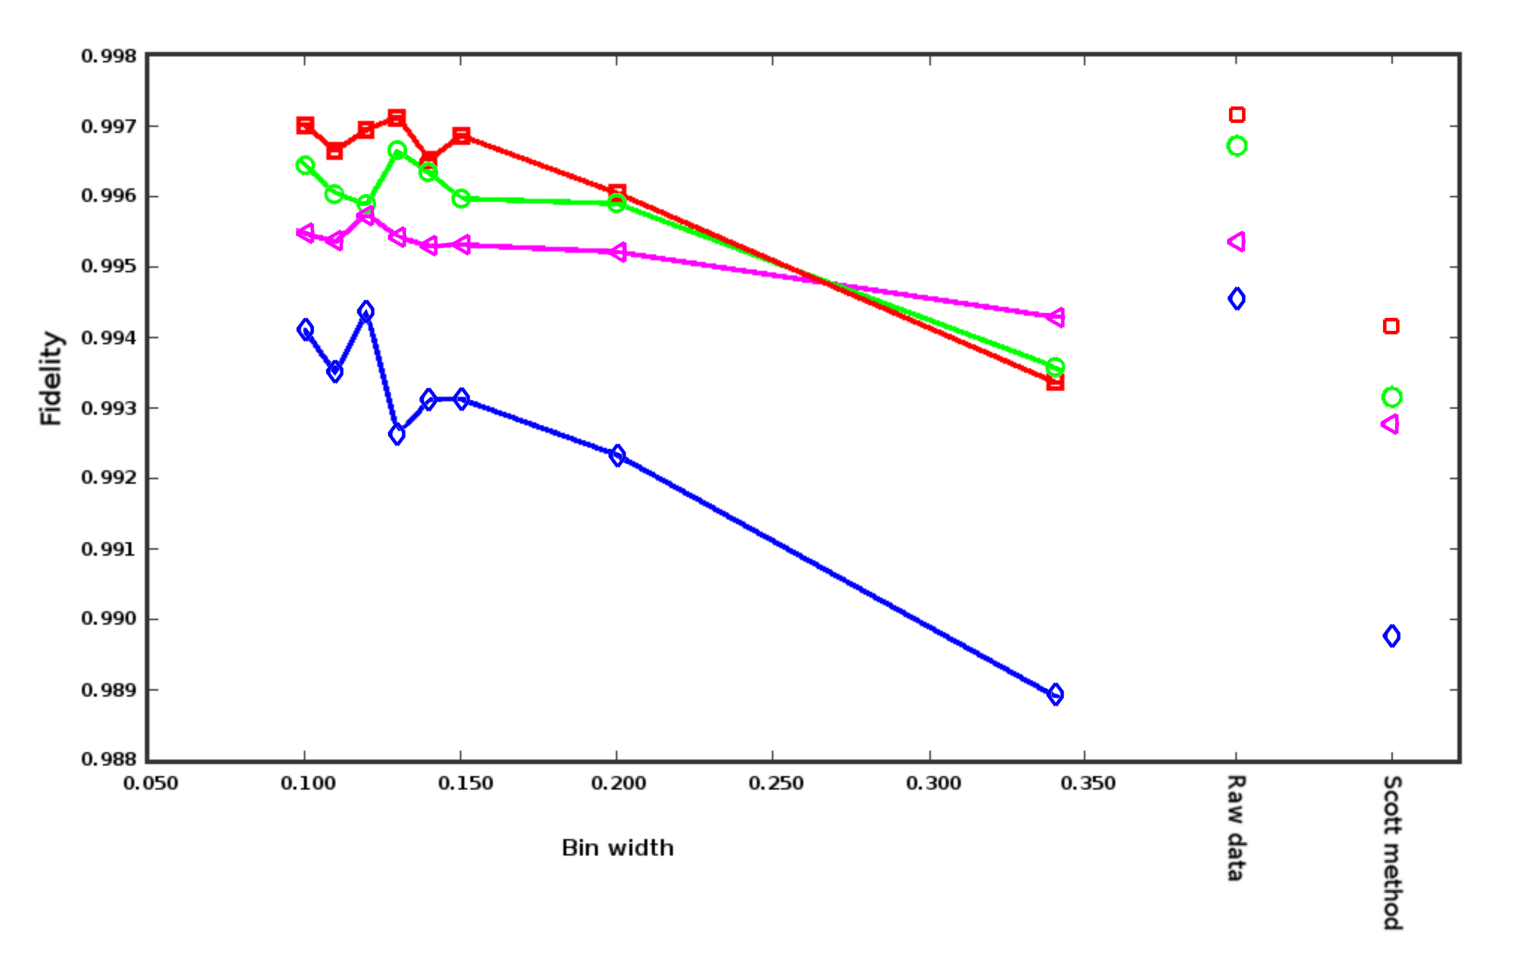
\includegraphics[width=0.5\textwidth]{methods_fidelity_singledata.eps}
  \caption{\SGs{Average} Fidelities as functions of the bin width for
    a cat state with amplitude $\alpha=1$ \SG{and photon loss
      ???}. The Hilbert space is truncated at $t=10$ photons. Each set
    of points with the same color and marker shape corresponds to a
    different data set. The mean bin width for Scott method is
    $0.35$.}
  \label{fig-methods_fidelity_singledata}
\end{figure}

%DISCUSSION OF FIGURE 2
%In Fig.~

%FIGURA 2
%\begin{figure}[h]
%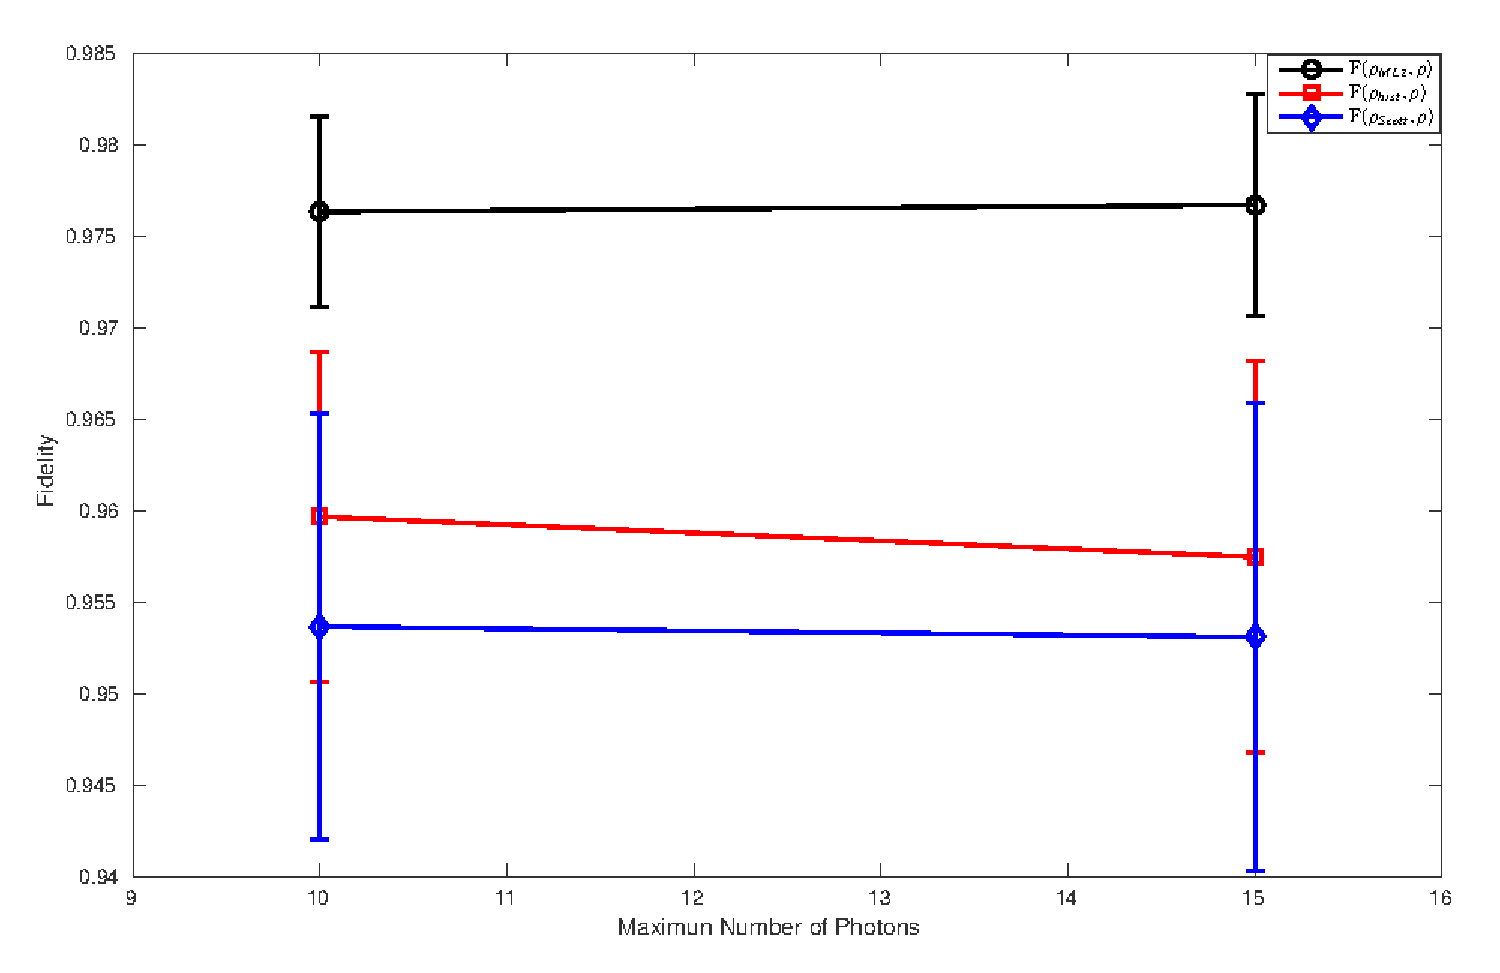
\includegraphics[width=0.49\textwidth]{FockState_(n=5).eps}
%\caption{}
%\label{fig-FockState_(n=5)}
%\end{figure}

%DISCUSSION OF FIGURE 2
The next set of results is presented in
Fig.~\ref{fig-fidelity_vs_binwidth_15_photons_catstate}, where we show
average fidelities as a function of the bin width for cat states with
amplitudes $\alpha=1$ and $\alpha=2$. The states are reconstructed in
a $t=15$ photons Hilbert space. \SG{The $\alpha=2$ state has
  probability of ??? to contain more than 15 photons.} The fidelity
for an $\alpha=1$ cat state is always greater than the fidelity for a
$\alpha=2$ cat state, including the case when we do not use
discretization. This is expected, because a $\alpha = 2$ state
requires more parameters to effectively describe its density matrix in
the photon number basis, so for a given amount of data, there is
greater statistical uncertainty.

The fidelity for the $\alpha = 2$ cat state decreases faster than the
fidelity for the $\alpha=1$ cat state as the bin size increases. This
is also expected because the $\alpha = 2$ state has more wiggles in
its probability distribution, so more information is lost when the
bins are larger. The average bin width used by Scott's method is
$0.35$ for the $\alpha=1$ cat state, and $0.64$ for the $\alpha=2$ cat
state, which results in significant fidelity loss. \SGs{The}
Leonhardt's width indicated in
Fig.~\ref{fig-fidelity_vs_binwidth_15_photons_catstate} is obtained by
using $t=15$\SGs{, the number of photons at which the Hilbert space is
  truncated,} \SG{in place of $n$ in} Eq.~(\ref{eq-leonhardt}).

% FIGURE 2
\begin{figure}
  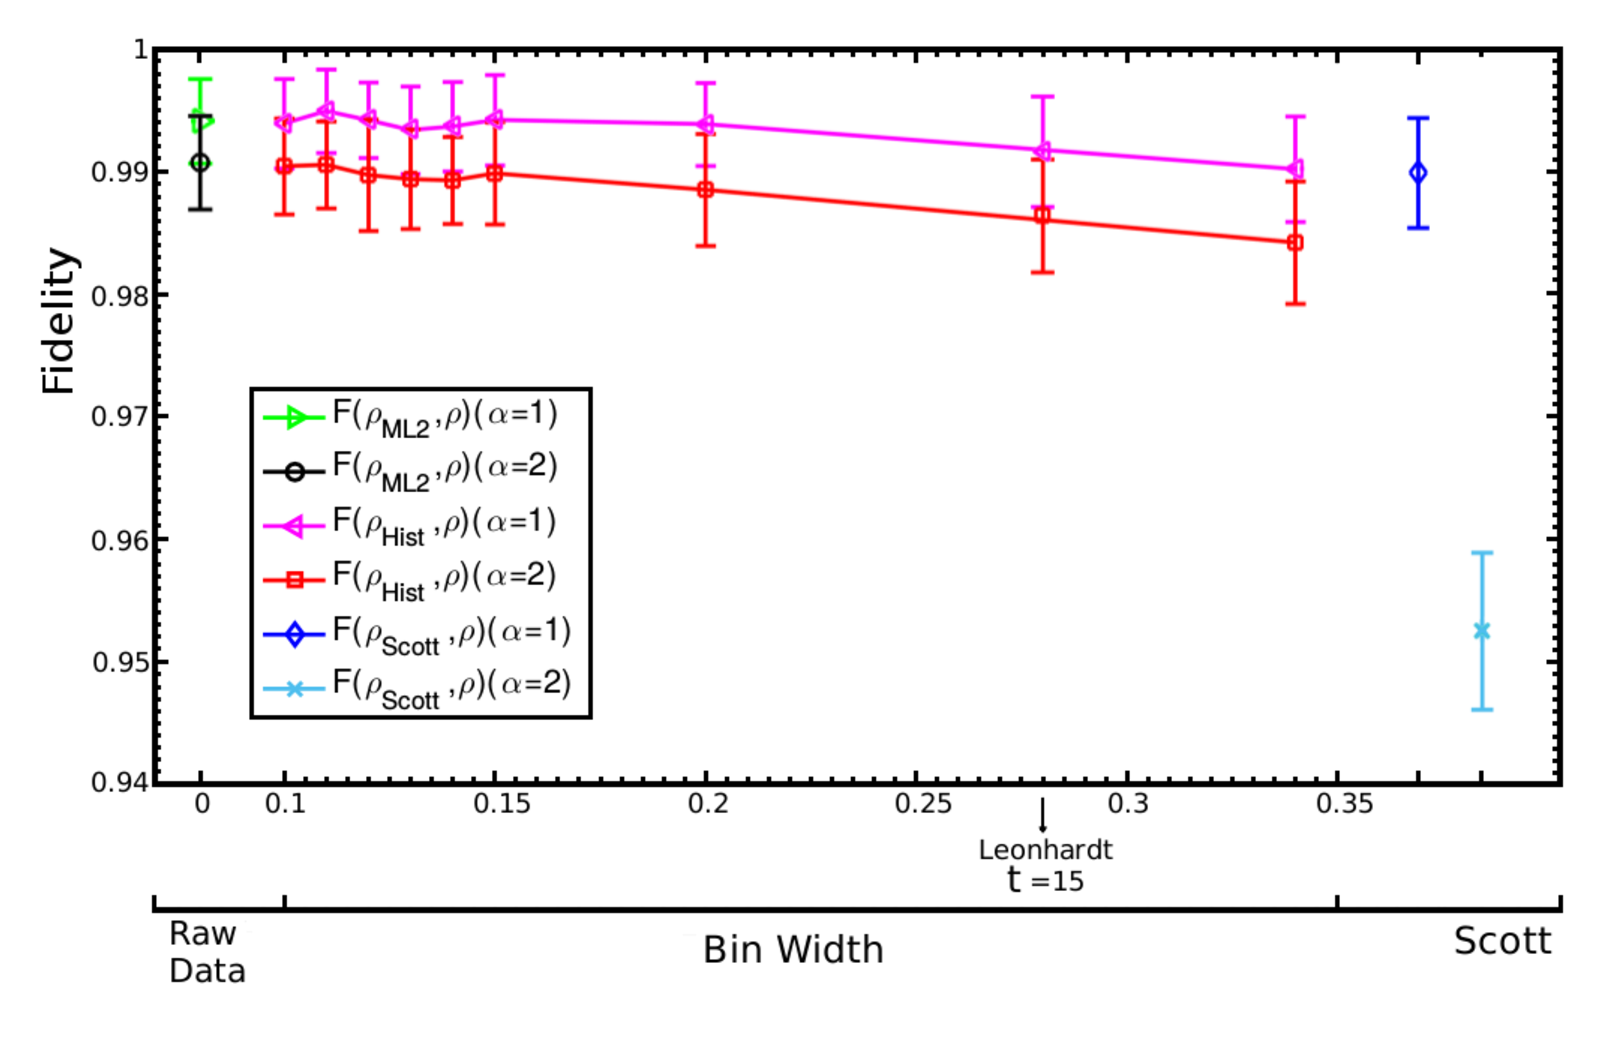
\includegraphics[width=0.49\textwidth]{catstate-alpha=1and2-15photons.eps}
  \caption{Average fidelity as a function of the bin width for cat
    states with amplitudes $\alpha=1$ and $\alpha=2$. The Hilbert
    space is truncated at $t=15$ photons. The mean bin widths for
    Scott's method are $0.35$ ($\alpha=1$ cat state) and $0.64$
    ($\alpha=2$ cat state).}
  \label{fig-fidelity_vs_binwidth_15_photons_catstate}
\end{figure}

% DISCUSSION OF FIGURE 3
%Figure~\ref{fig-squeezedvacuum_15_photons_Var=075} shows the
%average fidelity as a function of the bin width for a squeezed
%vacuum state whose squeezed quadrature has a variance 3/4 of the
%vacuum variance.  We use a 15 photon Hilbert space to reconstruct this
%state. In this graph, we extended the bin width to $1.05$ to show the 
%fidelity decreasing when the bin width increases. Using a bin width of
%$1.05$ gives us a fidelity loss of about 0.07, while the fidelitly 
%loss when we use Scott's optimal bin width (0.25) is of about $0.0002$.

%In Figs.~\ref{fig-fidelity_vs_binwidth_15_photons_catstate} and~\ref{fig-%squeezedvacuum_15_photons_Var=075}, we indicate the bin width obtained using Eq.~(\ref{eq-leonhardt}) for a maximum number of photon in the Hilbert space of $10$ and $15$, respectively. 

%FIGURE 3
%\begin{figure}
%  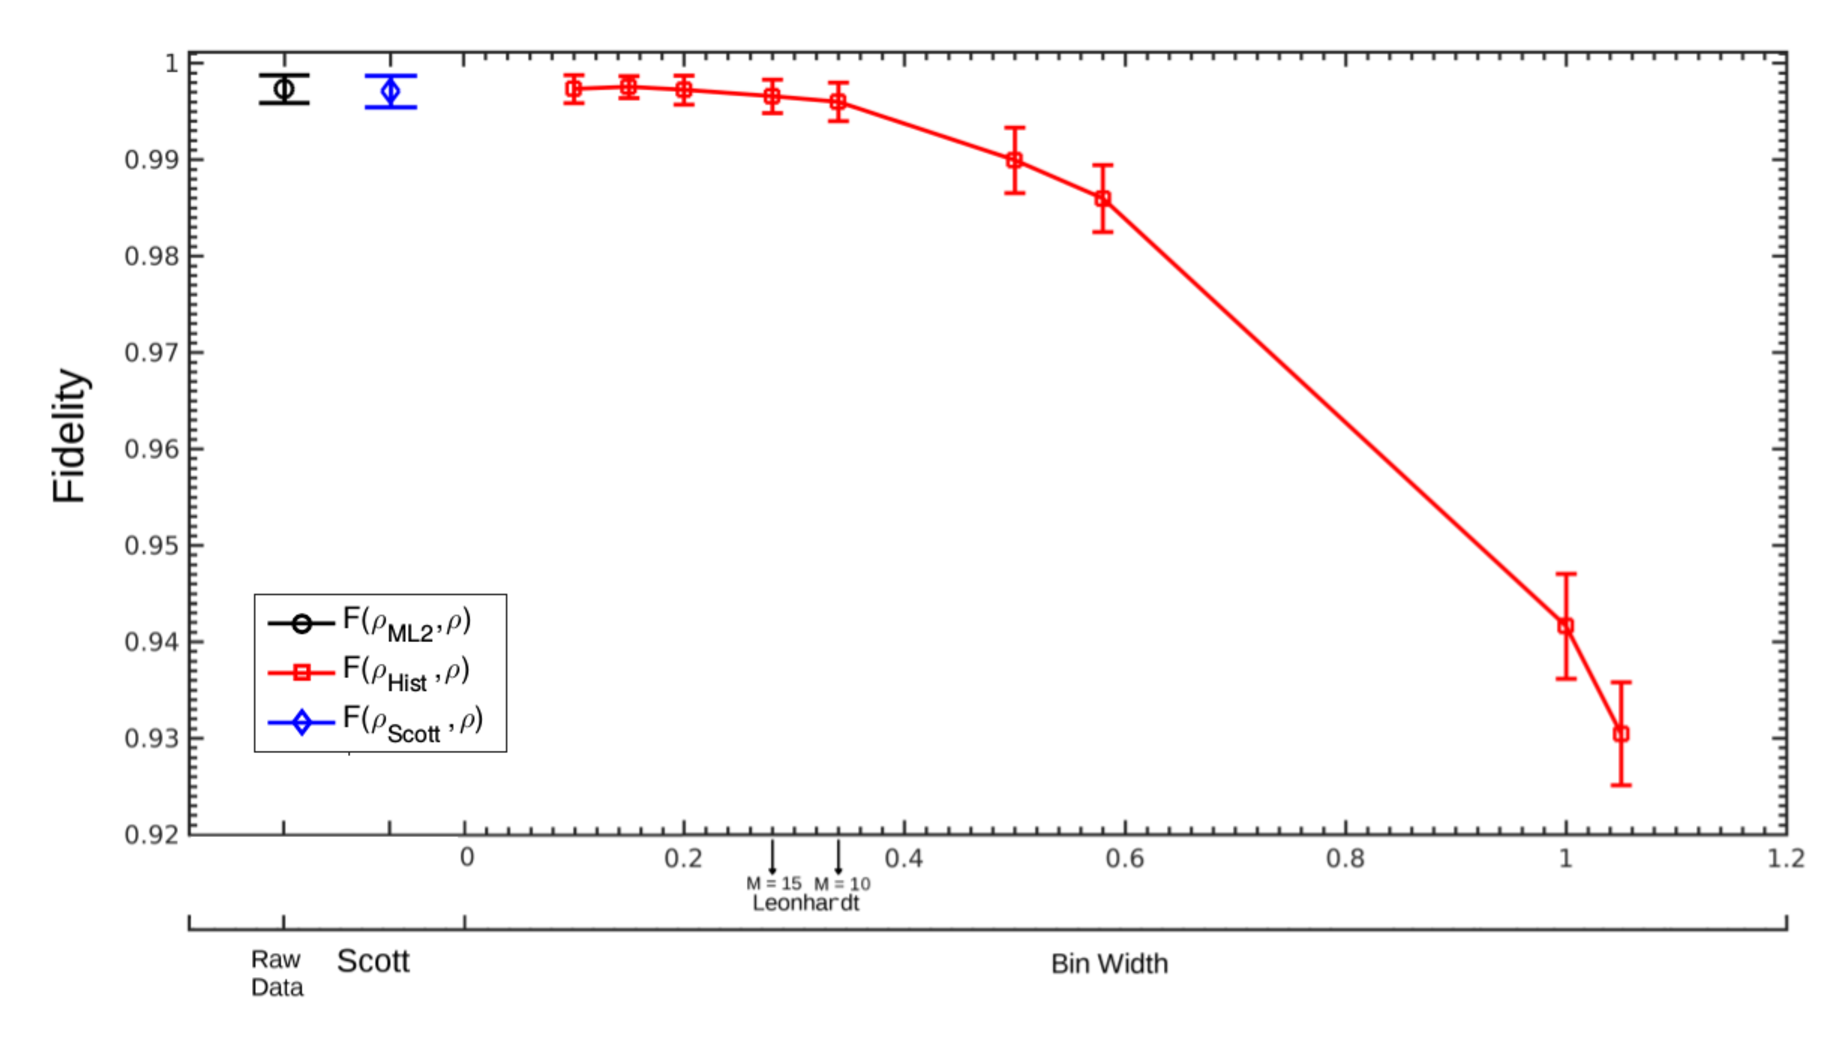
\includegraphics[width=0.49\textwidth]{squeezedvacuum-15photons-Var=075.eps}
%  \caption{Average fidelity as a function of the bin width for a
%    squeezed vacuum state whose squeezed quadrature has a variance 3/4
%    of the vacuum variance. The Hilbert space is truncated at 15
%    photons. The mean bin width for Scott's method is $0.25$.}
%  \label{fig-squeezedvacuum_15_photons_Var=075}
%\end{figure}

%DISCUSSION OF FIGURES 3, 4 AND 5
Until now, as mentioned before, every measurement outcome in a given
bin has been associated with the measurement operator for the
quadrature value at the center of that bin. Although this may be a
useful approximation for very small bins, to improve our analysis, we
now change each bin's measurement operator so that it represents a
measurement that occurs anywhere in the bin. \SGs{For that}\SG{To
  obtain these new operators}, we numerically integrate the
measurement operators over the width of each histogram bin. We
identify each case by adding $[$POVM-center$]$ and $[$POVM-integral$]$
to the legends in the graphs.

We also add to our analysis the use of the mean photon number estimate
in Leonhardt's formula, and we calculate the fidelity between
$\rhotrue$ and the state $\rho_{\mathrm{Leonhardt}}$ estimated using
the resulting bin width. Recall that Leonhardt recommends that the bin
width should be equal \SG{to} or smaller \SG{than} the one calculated
using the maximum photon number in Eq.~(\ref{eq-leonhardt}) but here
we use the \SG{estimate of the}\SGc{Is that correct?} mean photon
number instead.

\SGc{I am restructuring this so that there is less redundancy between
  the text and the figure captions.}
Figs.~\ref{fig-Fidelity_vs_binwidth_catstate_Mph_10_alpha_1}
and~\ref{fig-Fid_vs_binwidth_catstate_alpha_2_Mph_15} show average
fidelities as functions of the bin width for cat states with
amplitudes $\alpha=1$ and $\alpha=2$,
respectively. \SG{Fig.~\ref{fig-squeezed_vacuum_variance_075_Mph_10}
  examines a squeezed vacuum state whose squeezed quadrature has a
  variance 3/4 of the vacuum variance.  Note for the cat states, as
  $\alpha$ increases, Scott's bin width also increases, which is
  certainly undesirable because the quadrature distributions contain
  more fine structure.  These graphs show that integrating the
  measurement operators over the width of each bin considerably
  improves the fidelity for all cases. We can also see that
  Leonhardt's suggestion using the estimated mean photon number can be
  safely used as the upper bound for the bin width.}

% FIGURE 3
\begin{figure}
  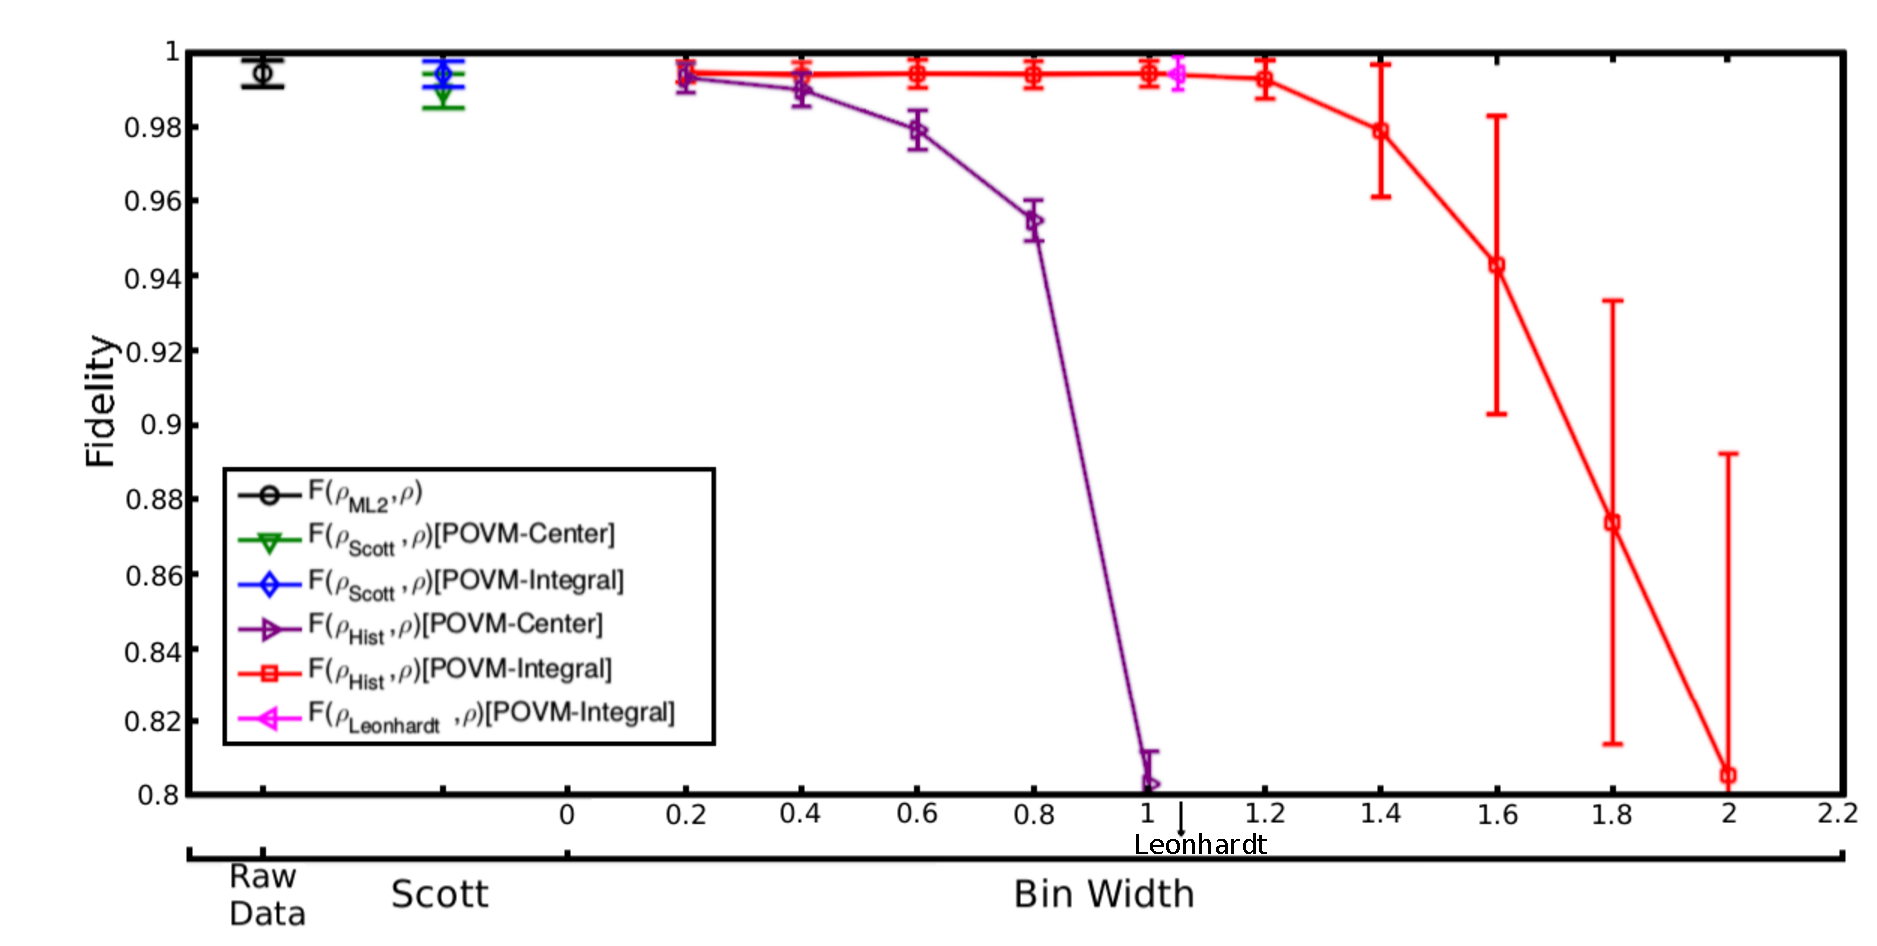
\includegraphics[width=0.49\textwidth]{catstate-alpha=1-10photons.eps}
  \caption{Average fidelity as a function of the bin width for a cat
    state with amplitude $\alpha = 1$. The Hilbert space is truncated
    at $t=10$ photons. \SG{For this state,
      $\langle n \rangle = 0.6093$, and} \SGs{the estimated mean
      number of photons is}
    $\overline{\langle \hat{n} \rangle}=0.6109$, giving a bin width by
    Leonhardt's formula of $1.05$.  \SGc{Can we get the little
      pointers to Leonhardt's bin width in these figures?} The mean
    bin width for Scott's method is $0.35$.}
  \label{fig-Fidelity_vs_binwidth_catstate_Mph_10_alpha_1}
\end{figure}

% FIGURE 4
\begin{figure}
  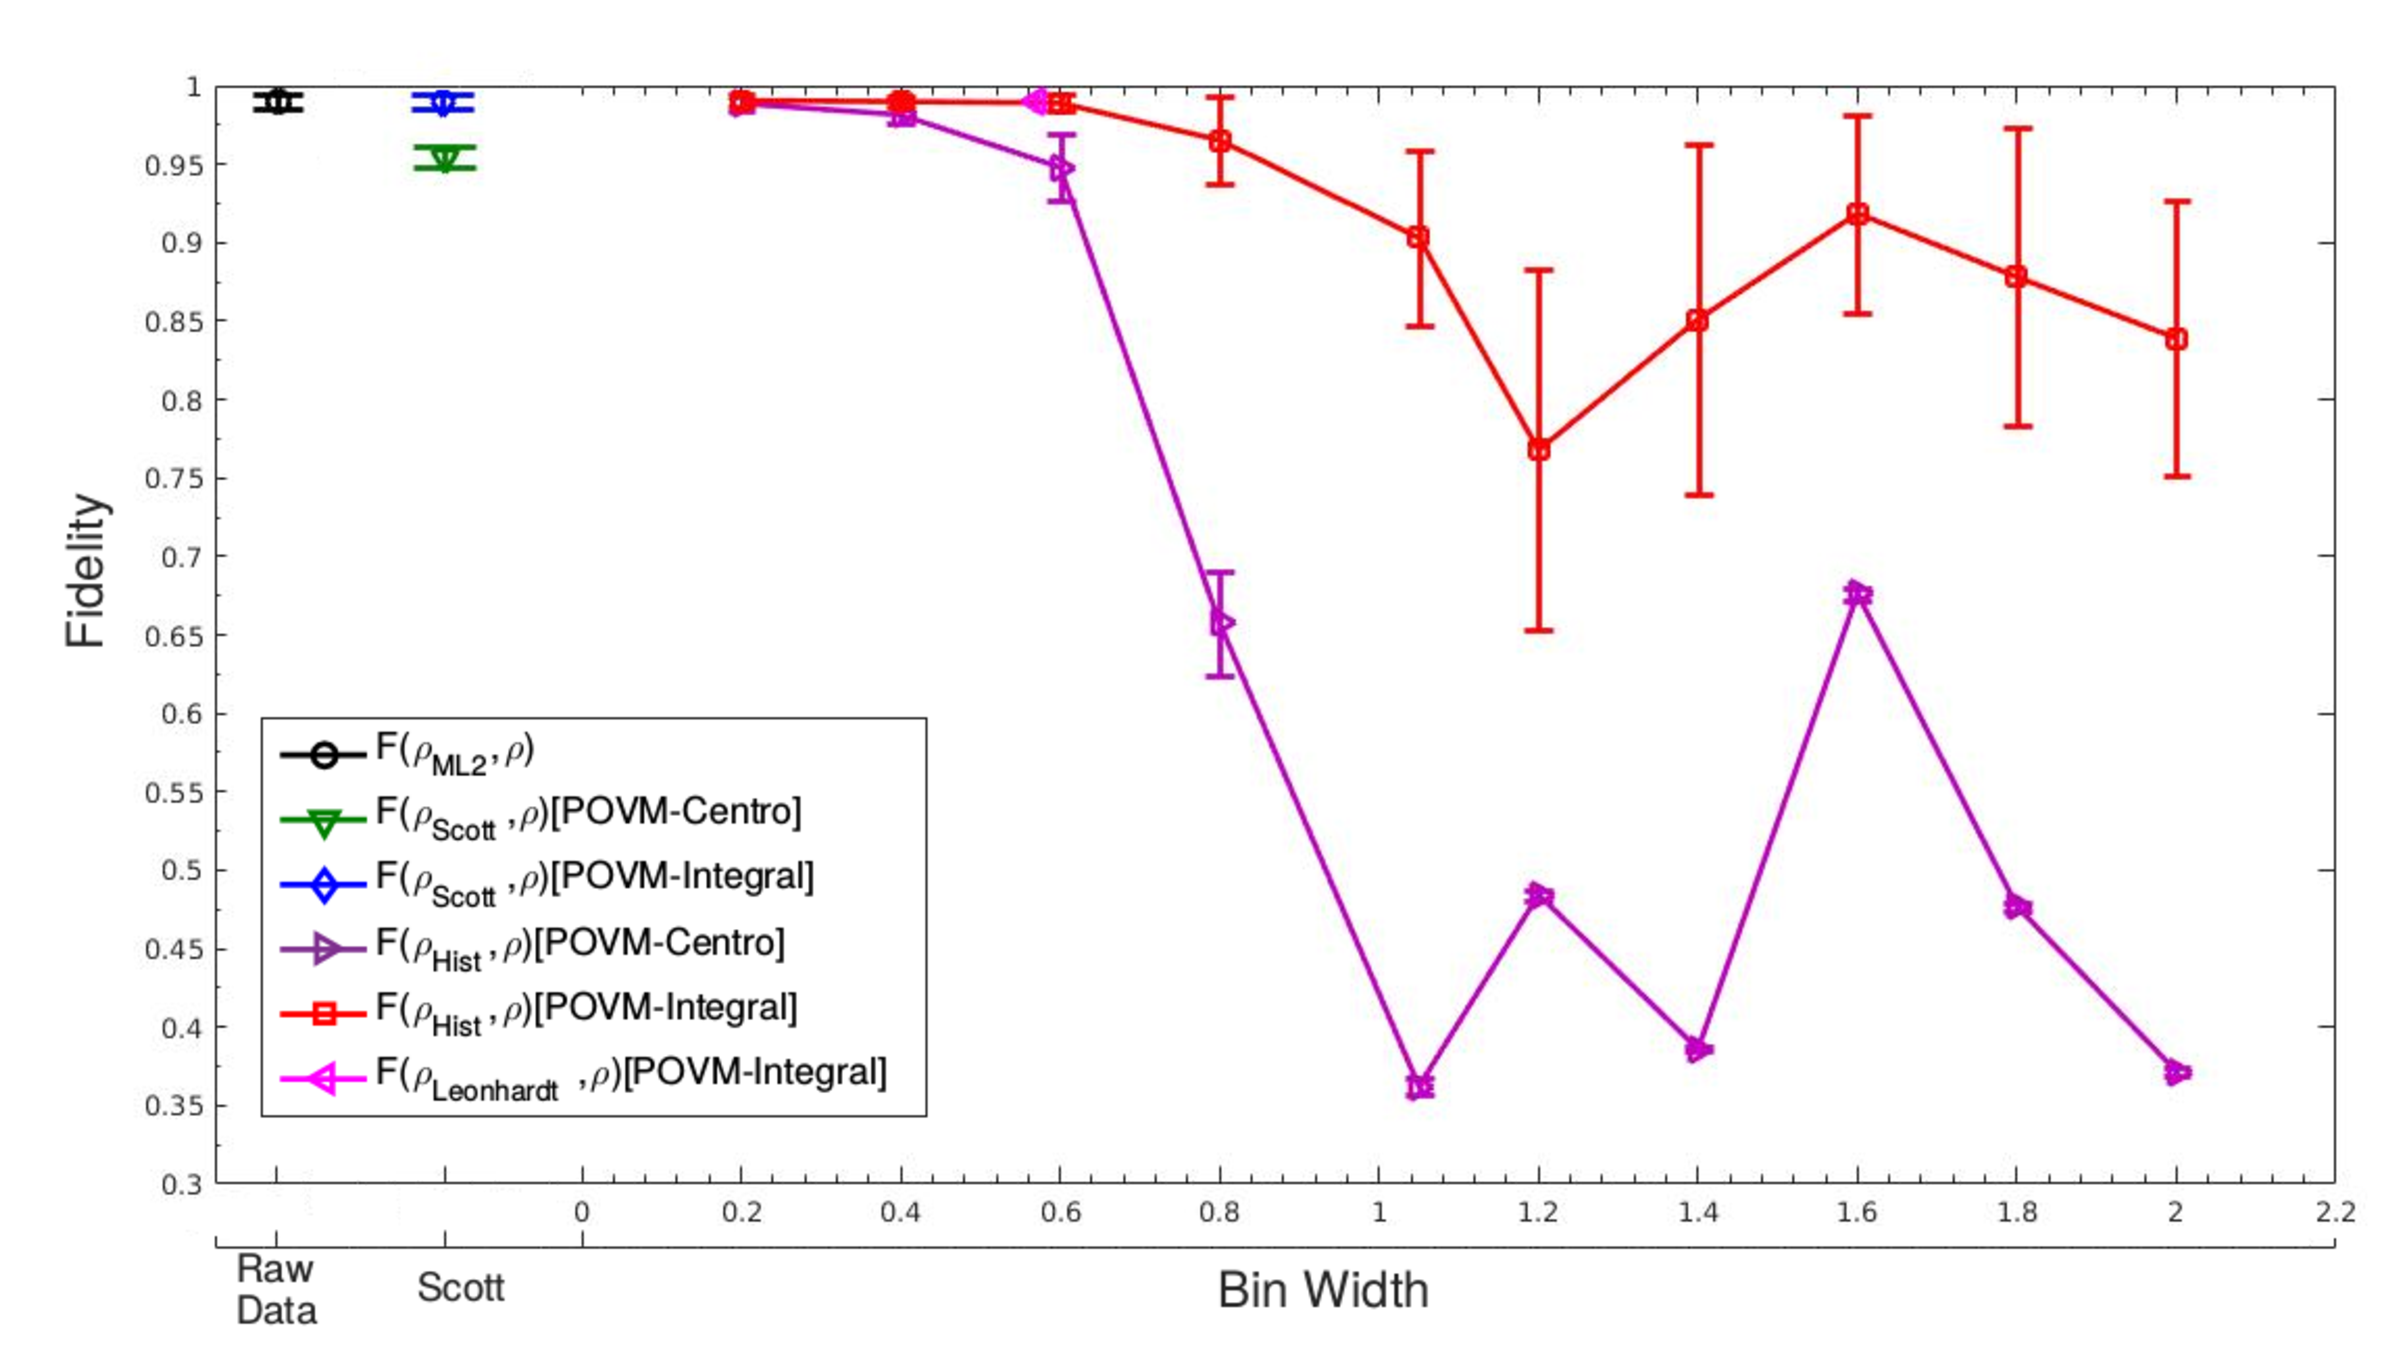
\includegraphics[width=0.49\textwidth]{catstate-alpha=2-15photons.eps}
  \caption{Average fidelity as a function of the bin width for a cat
    state with amplitude $\alpha = 2$. The Hilbert space is truncated
    at $t=15$ photons. \SG{For this state,
      $\langle n \rangle = 3.1978$, and} \SGs{the estimated mean
      number of photons is}
    $\overline{\langle \hat{n} \rangle}=3.1983$, giving a bin width by
    Leonhardt's formula of $0.58$.  The mean bin width for Scott's
    method is $0.64$.}
  \label{fig-Fid_vs_binwidth_catstate_alpha_2_Mph_15}
\end{figure}

% FIGURE 5
\begin{figure}
  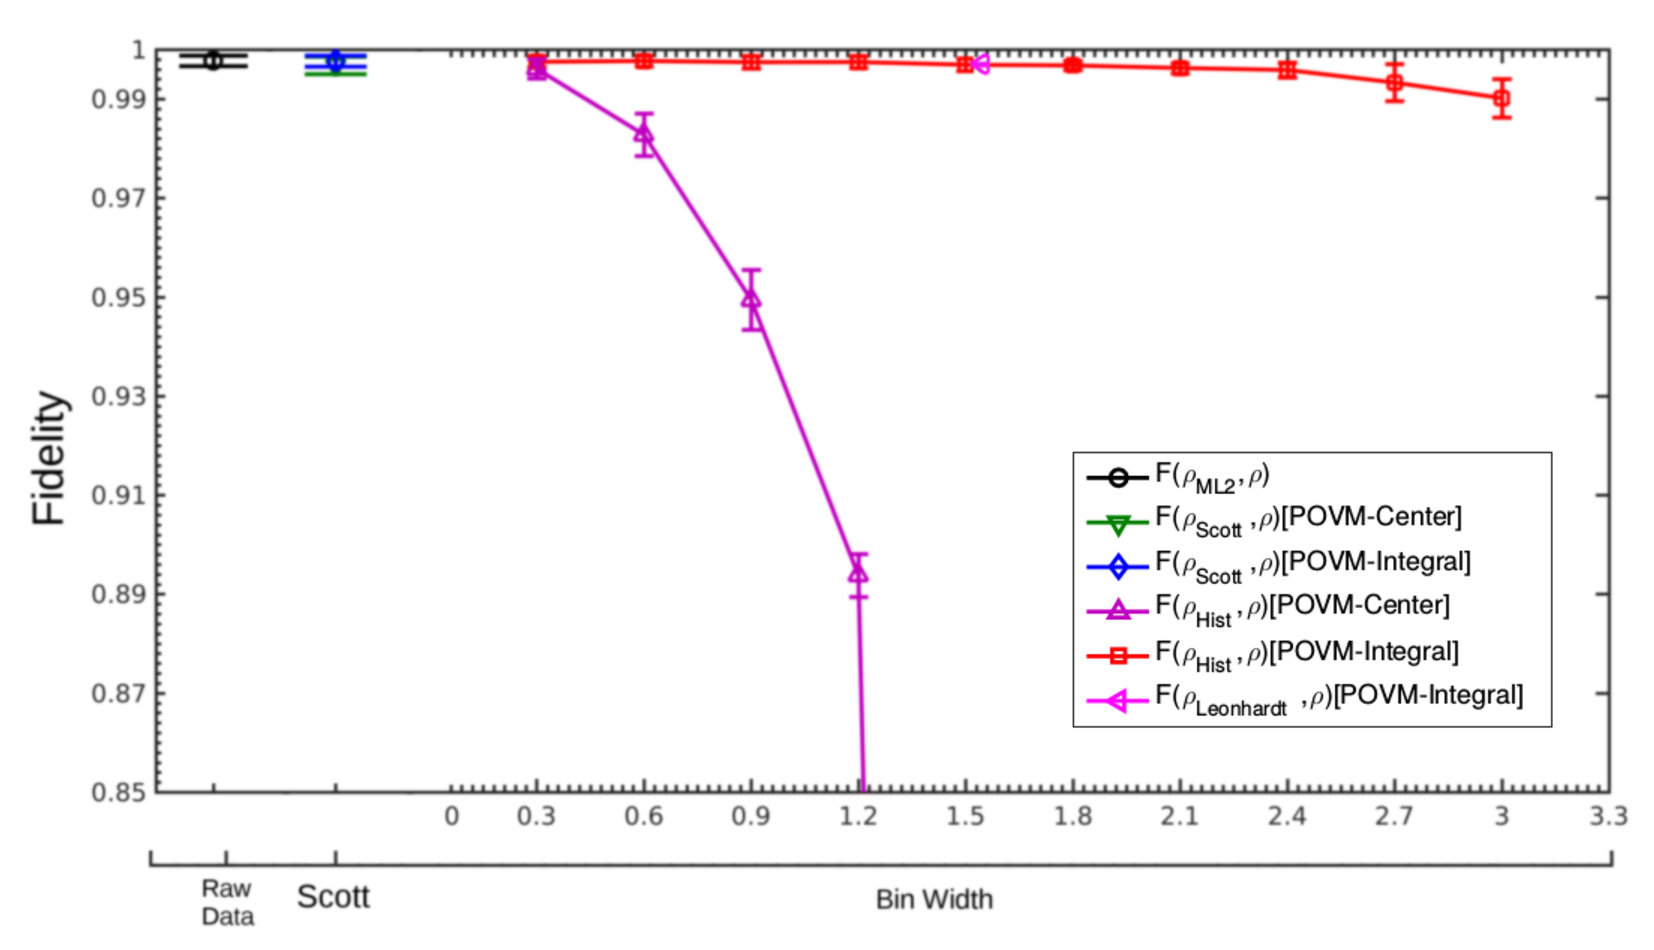
\includegraphics[width=0.49\textwidth]{squeezedvacuum-10photons-Var=075.eps}
  \caption{Average fidelity as a function of the bin width for a
    squeezed vacuum state whose squeezed quadrature has a variance 3/4
    of the vacuum variance. The Hilbert space is truncated at $t=10$
    photons.  \SG{For this state, $\langle n \rangle = 0.0167$, and}
    \SGs{the estimated mean number of photons is}
    $\overline{\langle \hat{n} \rangle}=0.0162$, giving a bin width by
    Leonhardt's formula of $1.54$.  The mean bin width for Scott's
    method is $0.25$.}
  \label{fig-squeezed_vacuum_variance_075_Mph_10}
\end{figure}

\SGs{For the $\alpha = 1$ cat state in
  Fig.~\ref{fig-Fidelity_vs_binwidth_catstate_Mph_10_alpha_1}, the
  estimated mean number of photons is
  $\overline{\langle \hat{n} \rangle}=0.6109$ (whereas the true mean
  number of photons is $0.6093$), which gives us, by Leonhardt's
  formula a bin width of $1.05$. For the $\alpha = 2$ cat state in
  Fig.~\ref{fig-Fid_vs_binwidth_catstate_alpha_2_Mph_15}, the
  estimated mean number of photons is
  $\overline{\langle \hat{n} \rangle}=3.1983$ (whereas the true mean
  number of photons is $3.1978$), giving a bin width of $0.58$. The
  squeezed vacuum state of
  Fig.~\ref{fig-squeezed_vacuum_variance_075_Mph_10} has an estimated
  mean number of photons of
  $\overline{\langle \hat{n} \rangle}=0.0162$ (whereas the true mean
  number of photons is $0.0167$), giving a bin width, by
  Eq.~(\ref{eq-leonhardt}), of $1.54$.}

\SG{All of the} \SGs{two} \SG{discretization} methods considered here
\SGs{, Leonhardt's and Scott's methods,} give \SG{much} faster
fidelity estimates, as we can see in Figs.~\ref{fig-time-catstate}
and~\ref{fig-time-squeezed}, with no significant loss of
\SGs{information}\SG{fidelity}. \SG{The times reported here include
  any calculations required to determine the desired bin width from
  the original homodyne data, the construction of histograms, and the
  ML density matrix estimation.} \SGc{We should briefly describe the
  computer used to make these graphs: what is its processor speed,
  number of cores, memory?}

% FIGURE 6
\begin{figure}
  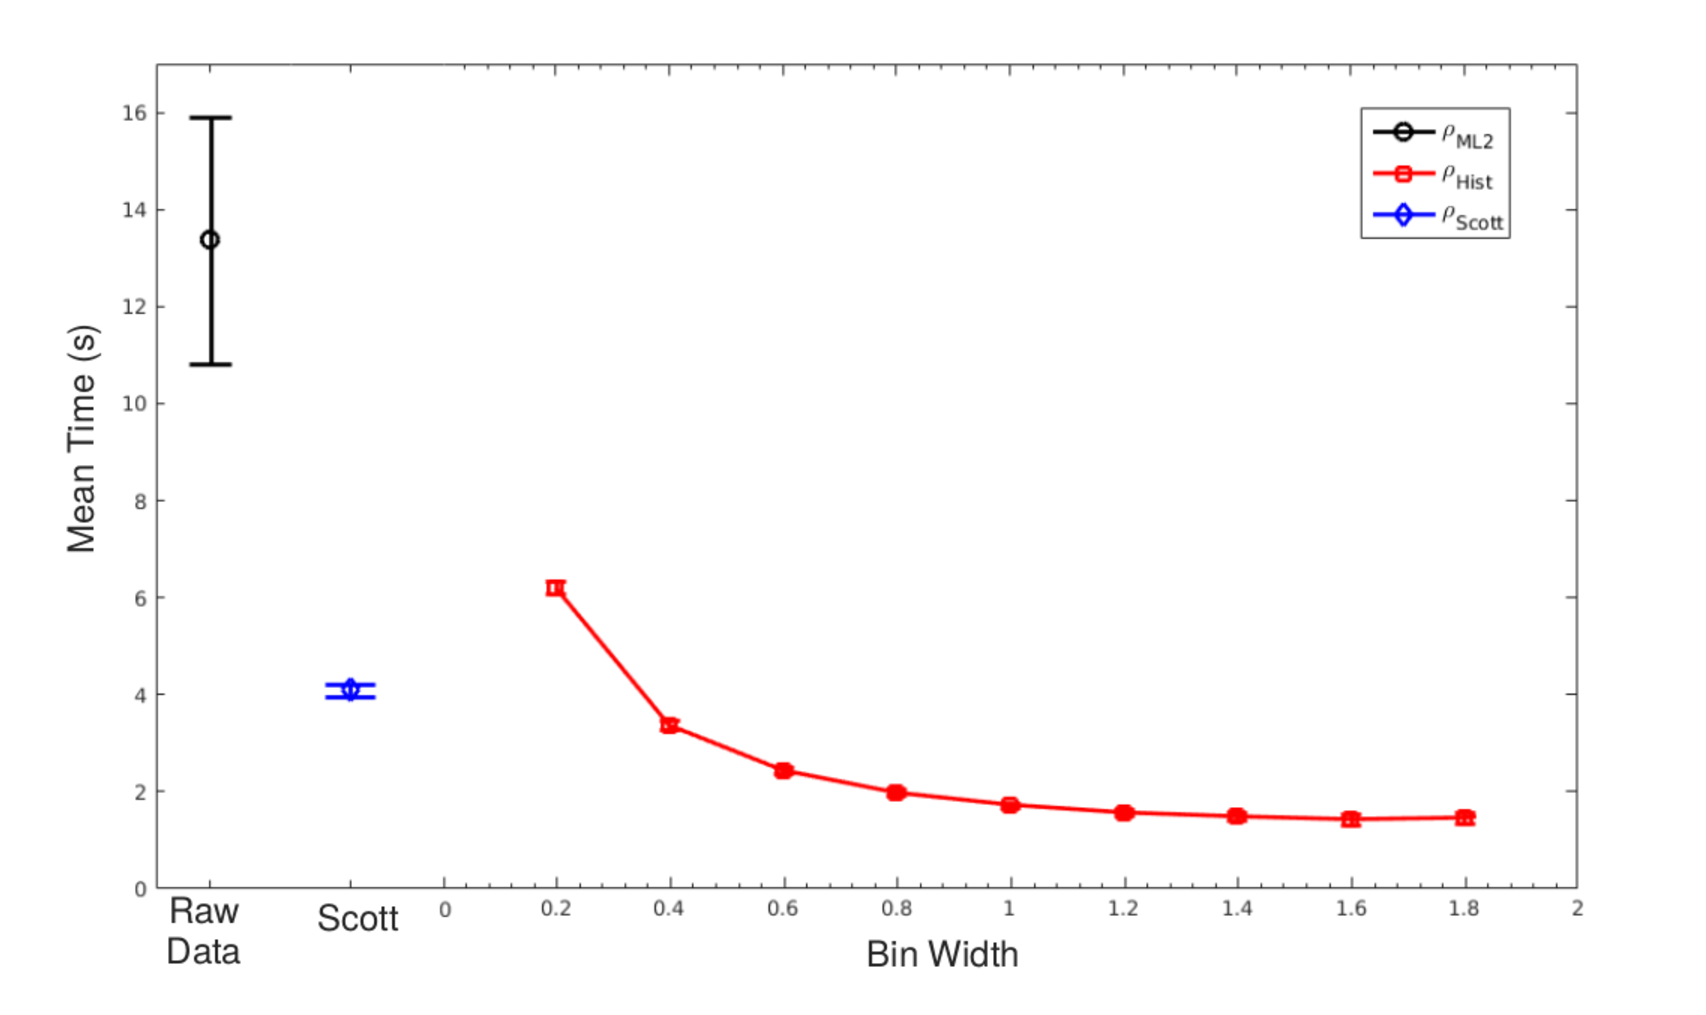
\includegraphics[width=0.49\textwidth]{time-estadogato_alpha_1.eps}
  \caption{Mean time as a function of the bin width for a cat state
    with amplitude $\alpha = 1$. The Hilbert space is truncated at $t=10$
    photons. The mean bin width for Scott's method is $0.35$, and the
    bin width given by Leonhardt's formula is $1.05$.}
  \label{fig-time-catstate}
\end{figure}

% FIGURE 7
\begin{figure}
  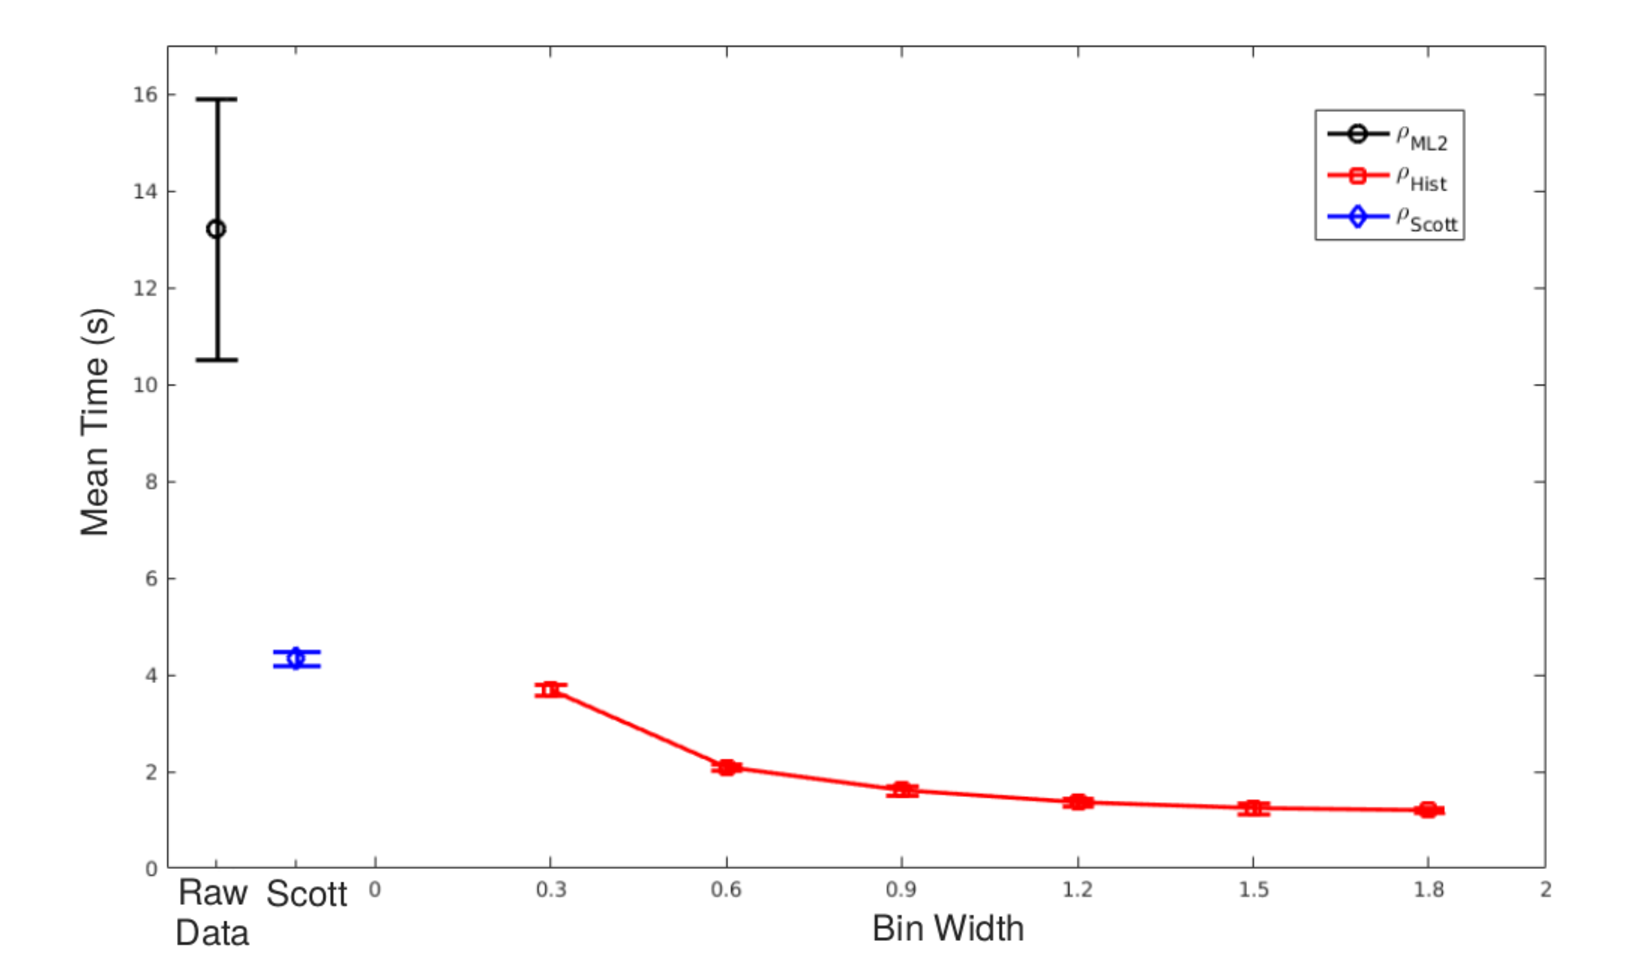
\includegraphics[width=0.49\textwidth]{time-vacuocomprimido.eps}
  \caption{Mean time as a function of the bin width for a squeezed
    vacuum state whose squeezed quadrature has a variance 3/4 of the
    vacuum variance. The Hilbert space is truncated at $t=10$ photons. The
    mean bin width for Scott's method is $0.25$, and the bin width
    given by Leonhardt's formula is $1.54$.}
  \label{fig-time-squeezed}
\end{figure}



\section{Conclusion}
\label{conclusion}

We have used idealized numerical experiments to generate simulated
data, performed maximum likelihood tomography on data sampled
from cat states and squeezed vacuum states with and without
discretization, and estimated the fidelities between
the reconstructed states and the true state. We used two different
methods to choose the bin width: Scott's and Leonhardt's methods. We
studied using measurement operators calculated using the
quadrature exactly at the center of each bin and integrating the
measurement operators along the length of the bin. 

Scott's method calculates an optimal bin width, for each phase, based
on the size and the standard deviation of the sample. Leonhardt's
method recommends a bin width narrower than $q_n/2$, where $q_n$
\SGs{depends on the}\SG{decreases with the square root of the} number
of photons in the state being reconstructed.  Since, in a real
experiment, we do not know the mean number of photons in the state
considered, we estimate the mean photon number from the quadrature
measurement results.

We have found that our proposed method to find the mean number of
photons from the quadrature measurement results gives accurate
results. We checked that by comparing the estimated mean number of
photons with the true mean number of photons for the cat states and
squeezed vacuum states. We also have found that integrating the
measurement operators over the width of each histogram bin
significantly improves the fidelity. Using this strategy, Leonhardt's
formula safely establishes an upper bound to the bin width, and both
methods provides a faster statistical estimation without losing too
much information.  \SGc{Do we have any cases in which Scott's method
  is really bad?}  \SGc{One might tailor Scott's rule using other
  distributions based on the state one expects to prepare in the
  experiment.}



\begin{acknowledgments}
  \HV{We thank ?????????????? for
    helpful comments on the manuscript.}  H. M. Vasconcelos thanks the
  Schlumberger Foundation's Faculty for the Future program for
  financial support. J. L. E. Silva thanks Coordena\c c\~ao de
  Aperfei\c coamento de Pessoal de N\'ivel Superior (CAPES) for
  financial support. This work includes contributions of the National
  Institute of Standards and Technology, which are not subject to
  U.S. copyright.
\end{acknowledgments}


% BibTeX users please use one of
%\bibliographystyle{spbasic}      % basic style, author-year citations
%\bibliographystyle{spmpsci}      % mathematics and physical sciences
%\bibliographystyle{spphys}       % APS-like style for physics
% Scott: My LaTeX does not know about spphys, but it is not necessary
% to specify a bibliography style.  revtex should authomatically use
% the correct style based on the documentclass.
\bibliography{histogram}   % name your BibTeX data base


% Non-BibTeX users please use%\begin{thebibliography}{}
%
% and use \bibitem to create references. Consult the Instructions
% for authors for reference list style.


%\end{thebibliography}


\end{document}

%%% Local Variables:
%%% mode: latex
%%% TeX-master: t
%%% End:
